\chapter{Implementación del prototipo}

\section{Estrategia reproducible}

La implementación se define en \code{infra/terraform}. En lugar de crear recursos manualmente y depender de memoria o capturas aisladas, el equipo conserva una descripción declarativa. Terraform compara esa descripción con el proveedor y presenta un plan antes de realizar cambios. La separación de archivos no altera el resultado, pero facilita la revisión: \code{network.tf} contiene VPC, subredes y rutas; \code{security.tf} contiene políticas; y \code{compute.tf} contiene recursos temporales.

\begin{figure}[H]
\centering
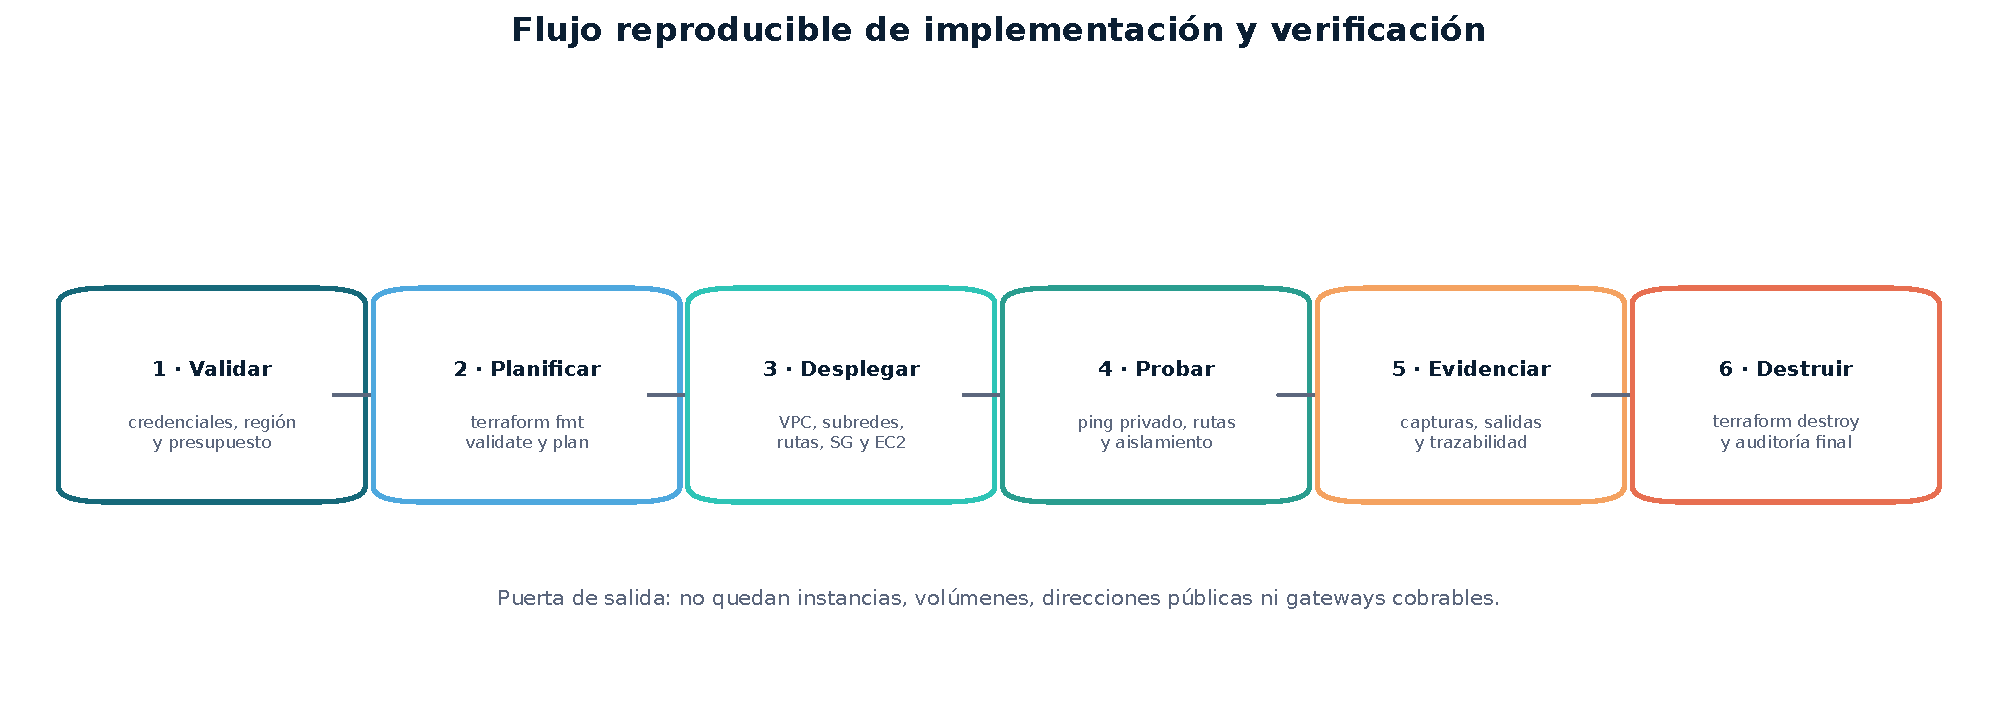
\includegraphics[width=\textwidth]{flujo-implementacion.pdf}
\caption{Flujo controlado para implementar, evidenciar y destruir. Elaboración propia.}
\label{fig:workflow}
\end{figure}

\section{Preparación}

\subsection{Identidad y región}

La identidad AWS debe pertenecer a una cuenta autorizada por el equipo. No se aceptan credenciales escritas dentro de archivos Terraform ni almacenadas en el repositorio. Antes de desplegar se verifica la identidad con un mecanismo de autenticación local, se confirma la región y se revisan los límites de servicio. La variable predeterminada es \code{us-east-1}, pero puede cambiarse sin alterar los CIDR.

El 20 de octubre de 2026 se verificó una sesión activa mediante \code{aws sts get-caller-identity} y se confirmó el perfil configurado en \code{us-east-1}. La Figura~\ref{fig:aws-identity-region} conserva los identificadores sensibles parcialmente ocultos y no muestra claves, tokens ni contraseñas.

\begin{figure}[H]
\centering
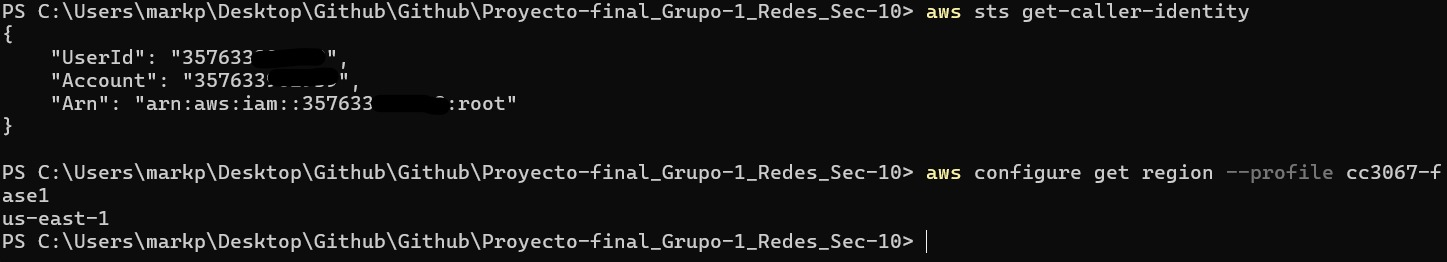
\includegraphics[width=0.96\textwidth]{aws-identidad-region-us-east-1.jpeg}
\caption{Verificación genuina de identidad AWS y región configurada. Los identificadores de cuenta fueron redactados antes de incorporarlos al informe.}
\label{fig:aws-identity-region}
\end{figure}

\begin{warningbox}[Control de privilegios]
La salida capturada identifica al principal raíz de la cuenta. Esta evidencia confirma acceso, pero no justifica usar privilegios raíz durante el despliegue. En la ventana de implementación debe preferirse un rol o usuario temporal con permisos limitados a los recursos del laboratorio.
\end{warningbox}

\subsection{Llave temporal}

La prueba necesita una llave SSH sólo durante la ventana de ejecución. El equipo genera el par fuera del repositorio, entrega a Terraform únicamente la ruta de la parte pública y protege la parte privada. Al destruir el entorno se elimina el recurso \code{aws\_key\_pair}; el archivo privado local se elimina mediante un procedimiento controlado después de verificar que ya no se necesita.

\subsection{Variables}

El archivo \code{terraform.tfvars.example} sirve de plantilla. \code{admin\_cidr} debe sustituirse por la IPv4 pública del operador con \code{/32}; \code{public\_key\_path} apunta a la llave pública temporal; y \code{enable\_compute=true} activa las tres instancias. El valor predeterminado es \code{false}, por lo que un uso descuidado no crea cómputo.

\section{Creación de la red}

La secuencia lógica es la siguiente:

\begin{enumerate}
  \item El proveedor consulta zonas disponibles y la AMI más reciente de Amazon Linux 2023.
  \item Se crea la VPC \code{10.10.0.0/24}, con DNS habilitado.
  \item Se crea un Internet Gateway y se adjunta a la VPC.
  \item Se crean cinco subredes canónicas en la primera zona disponible.
  \item Se crea una tabla pública con \code{0.0.0.0/0} hacia el gateway.
  \item Se crea una tabla privada sin salida predeterminada.
  \item Visitas y Administración se asocian con la tabla pública.
  \item Ventas, TI y Data Center se asocian con la tabla privada.
\end{enumerate}

Una tabla pública no asigna por sí sola direcciones públicas. La asignación automática mediante \path{map_public_ip_on_launch} permanece desactivada en todas las subredes. Únicamente el recurso del bastión solicita una dirección pública de manera explícita.

\section{Aplicación de seguridad}

Terraform crea dos grupos. El primero permite SSH desde la IP administrativa y salida sólo dentro de la VPC. El segundo permite SSH desde el grupo del bastión e ICMP entre sus propios miembros. Las dependencias se infieren a partir de las referencias entre recursos; por ejemplo, Ventas utiliza el identificador del grupo del bastión, no una cadena escrita manualmente.

\section{Creación del cómputo}

Con \code{enable\_compute=true}, se registra la llave pública, se crea un bastión en Administración y dos instancias en Ventas. Las tres usan volúmenes raíz GP3 de 8 GiB cifrados. El bastión recibe IP pública; las dos instancias de Ventas sólo reciben IP privadas. Las salidas de Terraform muestran la IP del bastión y la lista de IP privadas sin revelar secretos.

\section{Comandos de ejecución previstos}

\begin{Verbatim}[fontsize=\small,frame=single]
terraform init
terraform fmt -check -recursive
terraform validate
terraform plan -out=tfplan
terraform apply tfplan

# Después de capturar la evidencia:
terraform destroy
\end{Verbatim}

\begin{warningbox}[Nota sobre la ejecución final y el control de costos]
Las capturas incorporadas en esta versión demuestran que existe una identidad AWS configurada y que Terraform puede generar el plan de creación esperado. El equipo detuvo deliberadamente el procedimiento antes de \code{terraform apply} para evitar cargos por instancias EC2, almacenamiento y dirección IPv4 pública fuera de la ventana definitiva de pruebas.

La implementación real se realizará al final del proyecto, dentro de una única ventana corta y supervisada. En esa misma sesión se aplicará el plan, se capturarán la VPC, las subredes, las tablas de rutas, los grupos de seguridad y las instancias; se ejecutará el ping entre las dos instancias privadas de Ventas; y se destruirán todos los recursos inmediatamente después de conservar la evidencia. Por tanto, estas actividades representan compromisos de ejecución final y no resultados ya obtenidos.
\end{warningbox}
